\textbf{Beispiel 1} \\ \\
a)\\ \\
Hier müssen die Differentialgleichung inklusive der Randbedingungen sowohl für die Zylinderwand als auch für den Kunststoff aufgestellt werden. Für die Differentialgleichung wird die Form der Wärmeleitgleichung  für Zylinderkoordinaten verwendet. Über die allgemeine Form des Wärmeleitgesetz lassen sich die Randbedingungen herleiten. Da es sich hier um ein Problem handelt, bei denen die Zylinderkoordinaten verwendet werden lautet der Nabla-Operator
\[
	\nabla = \frac{\partial}{\partial r}\textbf{e}_r + \frac{1}{r}\frac{\partial}{\partial \varphi}\textbf{e}_{\varphi} + \frac{\partial}{\partial z}\textbf{e}_z
\]
Hier handelt es sich zusätzlich noch um ein ebenes Problem, welches nur vom Radius $r$ abhängt, worauf sich der Nabla-Operator vereinfacht.\\ \\
Zylinderwand:\\
\textit{Wärmeleitgleichung}:
\[
	\rho_z c_{p,z} \dot{T}_z(r,t) = \lambda_z \left( \frac{1}{r}\frac{\partial}{\partial r}\left( r \frac{\partial}{\partial r}T_z(r,t)\right)\right)
\]
\textit{Randbedingungen}:
\begin{align*}
	\dot{q}_{hz} = \lambda_z\frac{\partial}{\partial r}T_z(r,t)|_{r = r_o} \\
	\dot{q}_{zp} = - \lambda_z\frac{\partial}{\partial r}T_z(r,t)|_{r = r_i}
\end{align*}
\textit{Anfangsbedingung}:
\[
	T_z(r,0) = T_\infty
\]
\\
Polymer:\\
\textit{Wärmeleitgleichung}:
\[
	\rho_p c_{p,p}(T_p)\dot{T}_p =  \lambda_p \left( \frac{1}{r}\frac{\partial}{\partial r}\left( r \frac{\partial}{\partial r}T_p(r,t)\right)\right)
\]
\textit{Randbedingung}:
\[
		\dot{q}_{zp} = \lambda_z\frac{\partial}{\partial r}T_p(r,t)|_{r = r_i}
\]
\textit{Anfangsbedingung}:
\[
T_z(r,0) = T_\infty
\]
Wärmestromdichten für Randbedingungen:
\begin{align*}
	\dot{q}_{zp} &= \alpha_{zp} (T_z(r_i) - T_p(r_i)) \\
	\dot{q}_{hz} &= \alpha_{hz} (T_h - T_z(r_o)) \\
				 &= \frac{\alpha_{hz} / \alpha_\infty \frac{P}{A} + \alpha_{hz}(T_\infty - T_z(r_o))}{1 + \alpha_{hz} / \alpha_\infty}
\end{align*}
\newpage
b) \\ \\
\begin{figure}[h]
	\centering
	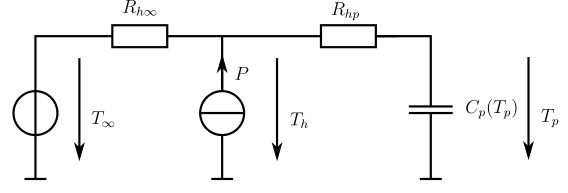
\includegraphics[width=12.5cm]{tikz/2_10_15_1b}
\end{figure}
\newline
Relevanten Größen:
\begin{align*}
	R_{h\infty} = \frac{1}{2r_o\pi L \alpha_\infty} \\
	C_p = r^2_i \pi L \rho_p c_{p,p}(T)
\end{align*}
und
\[
	R_{hp} = \frac{1}{2r_o\pi L k(r_o)}
\]
mit
\[
	k(r) = \frac{1}{r}\frac{1}{\frac{1}{\alpha_{hz}r_o} + \frac{1}{\lambda_z}\log\left( \frac{r_o}{r_i}\right) + \frac{1}{\alpha_{zp}r_i}}
\]
$k(r)$ wurde mit der Formel bei einer Wärmeleitung bei mehrschichtigen zylindrischen Wandaufbau aufgestellt.\\ \\
Einheiten:
\begin{align*}
	[R] &= KW^{-1} \\
	[C] &= JK^{-1} \\
	[P] &= W \\
	[T] &= K
\end{align*}
c) \\ \\
Die Differentialgleichung für die Ersatzschaltung lautet
\[
	\underbrace{(R_{hp} + R_{h\infty})C_p(T_p)}_{\tau(T_p)}\dot{T}_p = T_\infty + PR_{h\infty} - T_p
\]
Dadurch das $c_{p,p} = const$, wird die Differentialgleichung zu einer einfachen DGL 1.Ordnung.
Löst man diese erhält man die Lösung
\[
	T_p(t) = T_\infty + PR_{h\infty}(1 - exp(-t / \tau))
\]